\documentclass[crop,tikz]{standalone}
\usepackage{tikz}

\usetikzlibrary{positioning}

\tikzstyle{baseNode}=[draw,circle,minimum size=15pt,inner sep=0pt]
\tikzstyle{transition}=[-stealth, thick]

\begin{document}
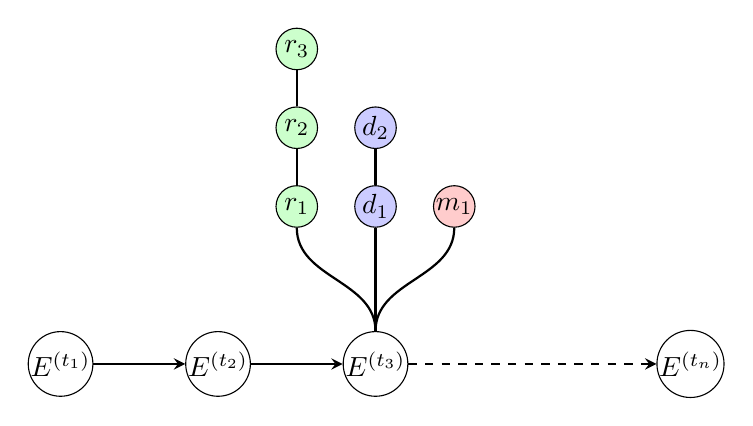
\begin{tikzpicture}

    \node[baseNode] (E1) at (0, 0) {$E^{(t_{1})}$};
    \node[baseNode] (E2) at (2, 0) {$E^{(t_{2})}$};
    \node[baseNode] (E3) at (4, 0) {$E^{(t_{3})}$};
    \node[baseNode] (En) at (8, 0) {$E^{(t_{n})}$};
    
    \node[baseNode,fill=green!20] (r1) at (3, 2) {$r_{1}$};
    \node[baseNode,fill=green!20] (r2) at (3, 3) {$r_{2}$};
    \node[baseNode,fill=green!20] (r3) at (3, 4) {$r_{3}$};
    
    \node[baseNode,fill=blue!20] (d1) at (4, 2) {$d_{1}$};
    \node[baseNode,fill=blue!20] (d2) at (4, 3) {$d_{2}$};
    
    \node[baseNode,fill=red!20] (m1) at (5, 2) {$m_{1}$};
    
    \draw[transition] (E1) to (E2);
    \draw[transition] (E2) to (E3);
    \draw[transition,dashed] (E3) to (En);
    
    \draw[thick] (E3) to[out=90,in=270] (r1);
    \draw[thick] (E3) to[out=90,in=270] (d1);
    \draw[thick] (E3) to[out=90,in=270] (m1);
    
    \draw[thick] (r1) to[out=90,in=270] (r2);
    \draw[thick] (r2) to[out=90,in=270] (r3);
    
    \draw[thick] (d1) to[out=90,in=270] (d2);

\end{tikzpicture}
\end{document}
